\documentclass[12pt,oneside,a4paper]{article}
\usepackage[table]{xcolor}
\usepackage{graphicx}
\usepackage{amsmath}
\usepackage{fancyhdr}
\usepackage{hyperref}
\usepackage{subfloat}
\usepackage{subfig}

\begin{document}

    \title{Rapport Q-Learning Space Invaders \\ \vspace*{3mm}G1 I0 M3 \large  \vspace*{7mm}\\ Étude de l'impact de $\gamma$ sur les résultats}

    \author{Julien Molinier, Maxime Leras}
    \date{7 Mai 2020}
    \maketitle\thispagestyle{empty}

    \newpage
    \clearpage
    \thispagestyle{empty}
    \renewcommand*\contentsname{Sommaire}
    \tableofcontents
    \newpage

    \pagestyle{fancy}
    \cfoot{\thepage}
    \fancyhead{}
    \fancyhead[R]{\leftmark}

    \pagenumbering{arabic}


    \section{Introduction}

    \paragraph{}
    Space Invaders est un jeu vidéo d'arcade sorti en 1978. Le principe
    est simple : détruire des vagues d'aliens se déplaçant horizontalement
    grâce à des tirs.
    Le Q-Learning est une technique d'apprentissage automatique
    interéssante pour ce type de jeu car elle ne nécessite aucun modèle
    initial de l'environnement.

    \paragraph{}
    Ce rapport a pour but d'étudier l'impact du paramètre $\gamma$ sur
    les résultats de l'apprentissage (facteur d'actualisation qui détermine
    l'importance des récompenses futures).


    \section{Description de l'environnement de jeu}

    \subsection{Description de l'état du jeu}

    \paragraph{}
    À chaque étape du jeu, gym atari renvoie 4 valeurs :
    L'objet \textit{observation} qui ici est une image à l'instant \textit{t}, le réel \textit{reward} qui
    prend différentes valeurs selon les bonnes ou mauvaises actions du joueur,
    le booléen \textit{done} qui détermine si la partie en cours est terminée ou non et
    le dictionnaire \textit{info} qui peut contenir des informations supplémentaires
    par exemple le nombre de vies restantes dans Space Invaders.\footnote{\url{https://gym.openai.com/docs/}}

    \subsection{Les récompenses}

    \paragraph{}
    Les récompenses par défaut pour \textit{SpaceInvaders-v0} sont uniquement positives.
    Elles sont de 5 pour les aliens de la ligne la plus proche du bas et augmentent de 5 par ligne.
    Un bonus violet apparaît parfois au dessus des aliens et donne 200 s'il est touché.

    Nous avions pensé ajouter une récompense négative dans le cas d'une vie perdue afin de peut-être
    permettre un lien entre les tirs des aliens et le fait de perdre. Nous pensions aussi lisser les
    récompenses notamment le bonus qui est très rare et crée des fortes croissances dans les scores sans que
    le lien \textit{action/reward} ne puisse être fait.

    \newpage

    \subsection{Traitement des données}

    \paragraph{}
    La donnée en entrée est une image de 210 par 160 (160 pixels en horizontal et 210 en vertical)
    en couleur. Afin de réduire cette entrée, nous avons réduit la taille de cette image.
    l'image au strict nécessaire de 80x80 pixels en noir et blanc. Nous avons fait le choix
    de ne garder qu'un seul pixel sur 2 en vertical car aucun déplacement vertical n'est possible et
    les tirs d'aliens restent visibles car bien plus longs que 2 pixels (voir Figure 1). Pour les pixels en abscisse,
    nous avons du garder la totalité des pixels et non pas un sur deux car les tirs
    ne font qu'un pixel de large et pourraient être totalement invisible s'ils sont sur un pixel impair.

    \begin{figure}[h]
        \centering
        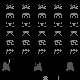
\includegraphics[width=0.5\textwidth] {./processed_image.png}
        \caption{Image après traitement}
    \end{figure}


    \section{Etude du paramètre $\gamma$}
    \newpage

    \subsection{Evolution du score moyen}
    \begin{figure}[hbt!]
        \centering
        \subfloat[$\gamma$ = 0.99]{
            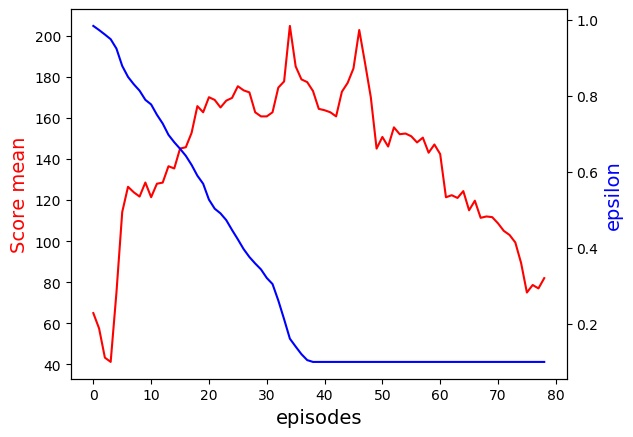
\includegraphics[width=0.3\textwidth] {./meanScore0.99.jpg}
        }
        \subfloat[$\gamma$ = 0.97]{
            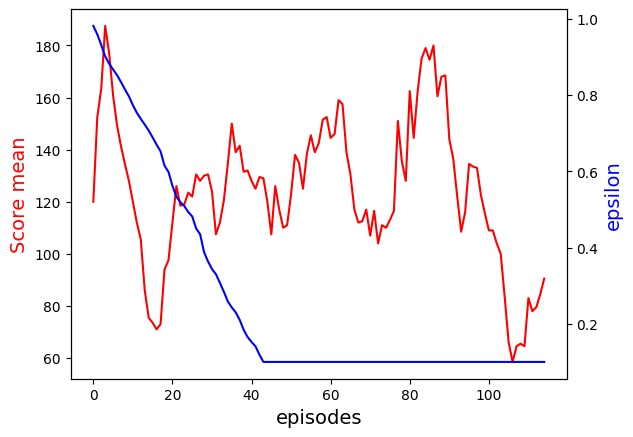
\includegraphics[width=0.3\textwidth] {./meanScore0.97.jpg}
        }
        \subfloat[$\gamma$ = 0.95]{
            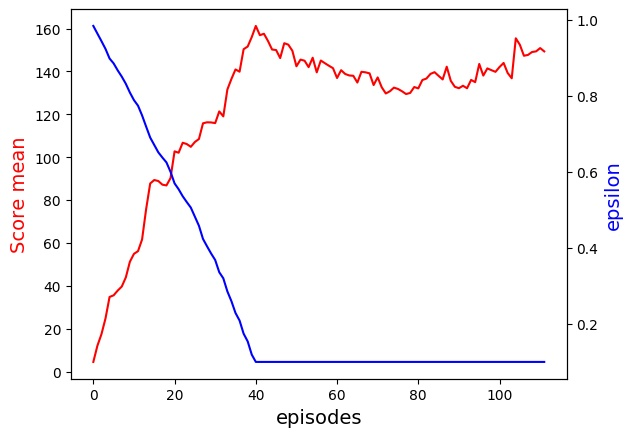
\includegraphics[width=0.3\textwidth] {./meanScore0.95.jpg}
        }
        \hspace{0mm}
        \subfloat[$\gamma$ = 0.9]{
            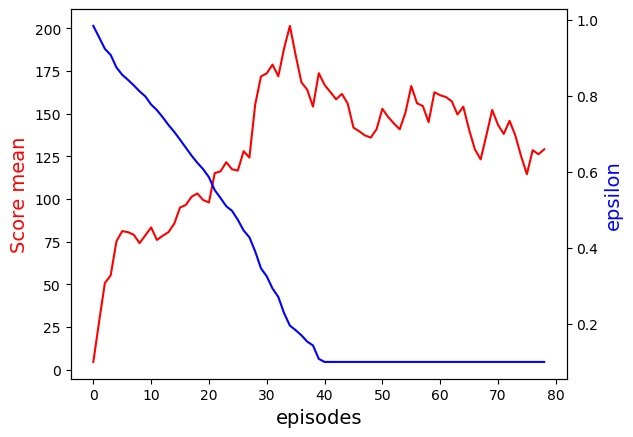
\includegraphics[width=0.3\textwidth] {./meanScore0.9.jpg}
        }
        \subfloat[$\gamma$ = 0.8]{
            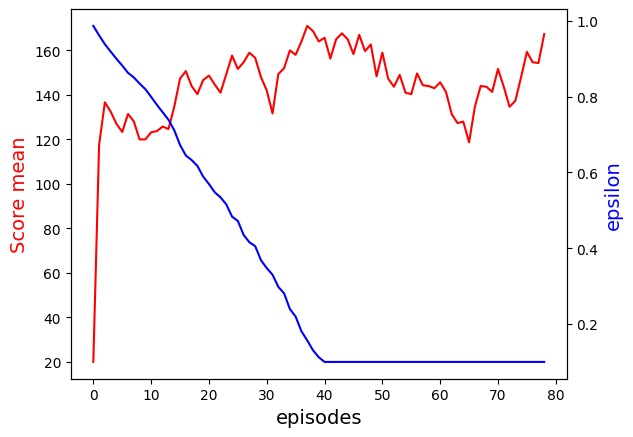
\includegraphics[width=0.3\textwidth] {./meanScore0.8.jpg}
        }
        \subfloat[$\gamma$ = 0.5]{
            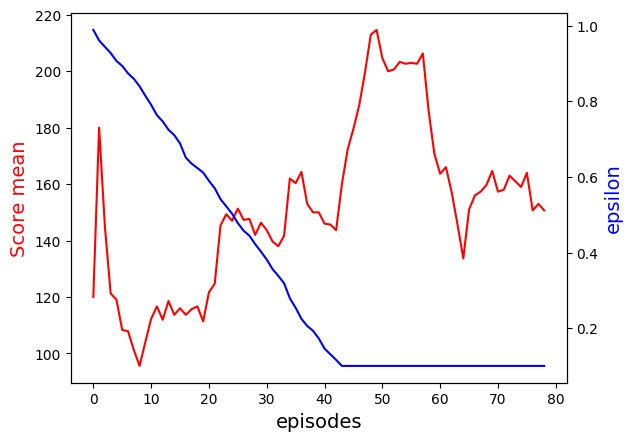
\includegraphics[width=0.3\textwidth] {./meanScore0.5.jpg}
        }
        \hspace{0mm}
        \subfloat[$\gamma$ = 0.3]{
            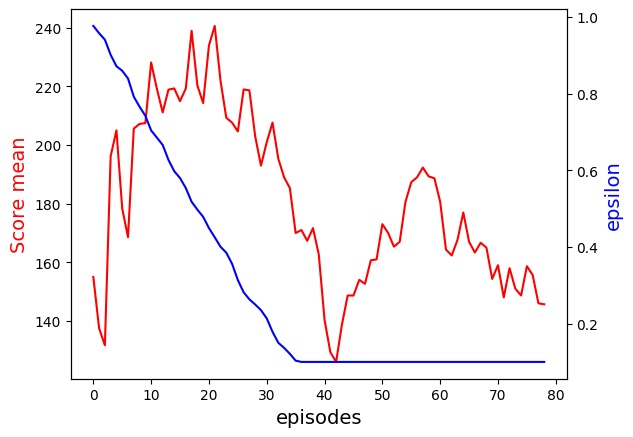
\includegraphics[width=0.3\textwidth] {./meanScore0.3.jpg}
        }
        \subfloat[$\gamma$ = 0.1]{
            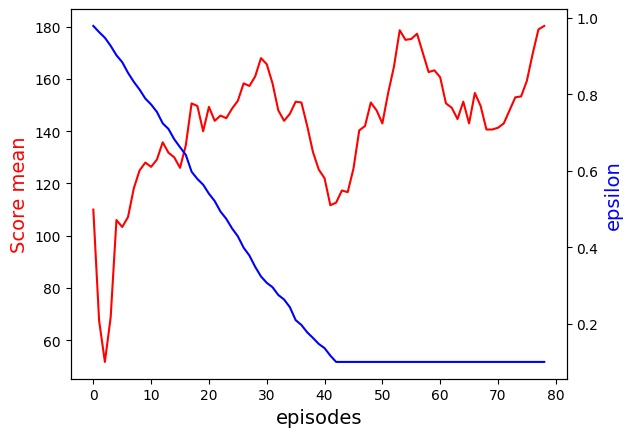
\includegraphics[width=0.3\textwidth] {./meanScore0.1.jpg}
        }
        \caption{Moyennes en fonction de $\gamma$}
    \end{figure}

    \paragraph{}
    Les graphiques ci-dessus montrent qu'un $\gamma$ trop proche de 1 a tendance à faire diverger la
    valeur de $\mathrm{Q}$ et donc le score moyen diminue plus le nombre d'épisode augmente car les valeurs sont lisées
    par l'effet de la loi des grands nombres. Un gamma trop petit (et donc de plus en plus proche de 0)
    rend l'agent myope aux récompenses courantes et donc les résultats sont tout aussi instables. D'après la figure 2,
    les courbes les moins bruitées et traduisant une forme d'apprentissage efficace sont celles où
    $0.8 \leq \gamma \leq 0.95$.
    \newpage

    \subsection{Evolution du score par partie}
    \begin{figure}[hbt!]
        \centering
        \subfloat[$\gamma$ = 0.99]{
            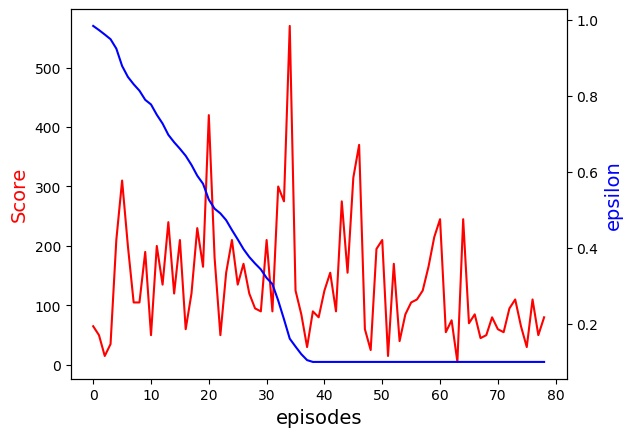
\includegraphics[width=0.3\textwidth] {./episode_score0.99.jpg}
        }
        \subfloat[$\gamma$ = 0.97]{
            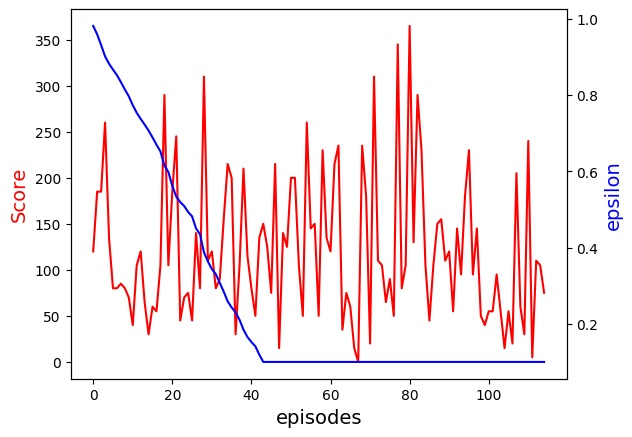
\includegraphics[width=0.3\textwidth] {./episode_score0.97.jpg}
        }
        \subfloat[$\gamma$ = 0.95]{
            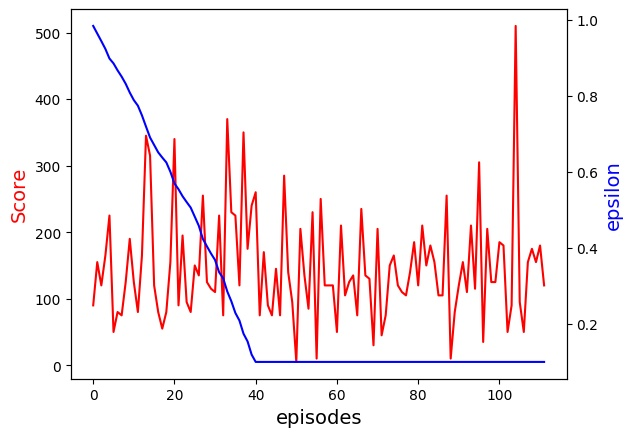
\includegraphics[width=0.3\textwidth] {./episode_score0.95.jpg}
        }
        \hspace{0mm}
        \subfloat[$\gamma$ = 0.9]{
            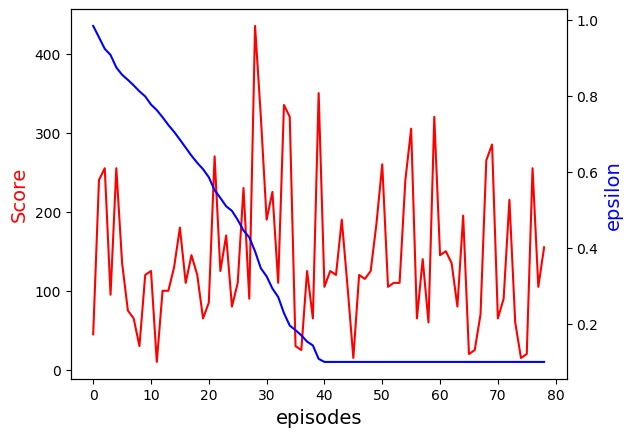
\includegraphics[width=0.3\textwidth] {./episode_score0.9.jpg}
        }
        \subfloat[$\gamma$ = 0.8]{
            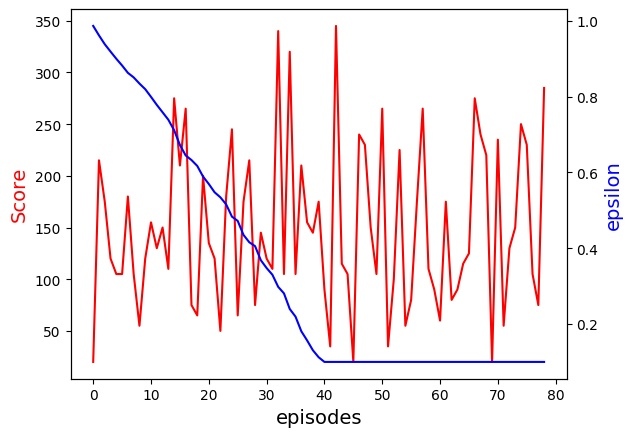
\includegraphics[width=0.3\textwidth] {./episode_score0.8.jpg}
        }
        \subfloat[$\gamma$ = 0.5]{
            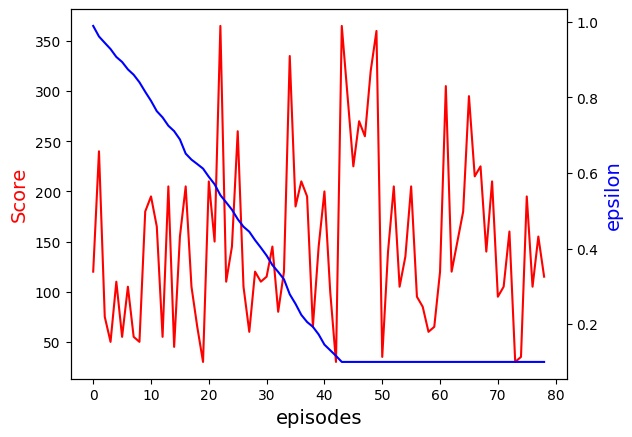
\includegraphics[width=0.3\textwidth] {./episode_score0.5.jpg}
        }
        \hspace{0mm}
        \subfloat[$\gamma$ = 0.3]{
            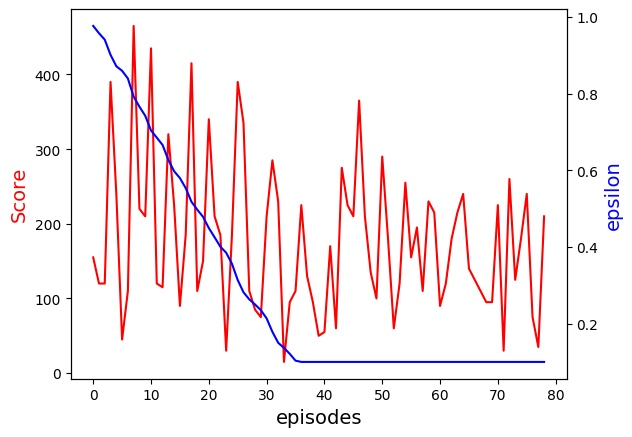
\includegraphics[width=0.3\textwidth] {./episode_score0.3.jpg}
        }
        \subfloat[$\gamma$ = 0.1]{
            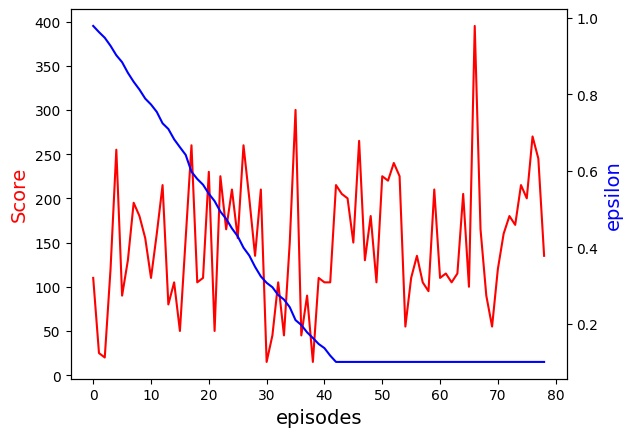
\includegraphics[width=0.3\textwidth] {./episode_score0.1.jpg}
        }
        \caption{Score en fonction de $\gamma$ (suite)}
    \end{figure}

    \newpage

    \subsection{Phénomène d'oubli catastrophique}

    \paragraph{}
    L'oubli catastrophique est un phénomène problématique des réseaux de neuronnes artificiels (ANN).
    \textit{Lors d’un nouvel apprentissage, un réseau
    de neurones artificiels modifie ses poids synaptiques en fonction
    de la nouvelle information et perd l’information précédemment
    apprise.}\footnote{\url{http://www.gdr-isis.fr/neurostic/wp-content/uploads/2019/10/Reyboz_NeuroSTIC2019.pdf}}
    Nous pouvons clairement observer ce phénomène dans les expériences décrites précédemment.
    \begin{figure}[h]
        \centering
        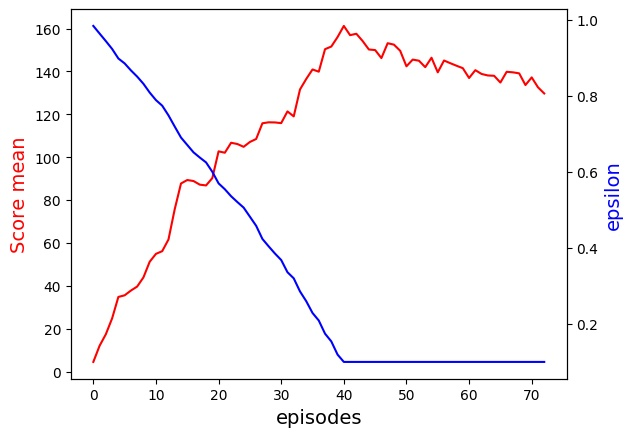
\includegraphics[width=0.5\textwidth] {./catastrophic_forgetting.jpg}
        \caption{Illustration du phénomène}
    \end{figure}

    \paragraph{}
    La figure ci-dessus montre clairement une perte d'information lors des épisodes qui suivent la 40ème itération.
    De plus on peut observer que la 40ème étape correspond au moment où $\epsilon$ attend sa valeur la plus basse
    avec 10\% de chance qu'une action soit liée au hasard.

    \paragraph{}
    Des solutions ont pu être développé pour limiter ce phénomène avec les avancées de la neuroscience. La première
    est l'algorithme EWC (Elastic Weight Consolidation) developpé par la société DeepMind\footnote{\url{https://deepmind.com/}}.
    La seconde est fondée sur le fonctionnement du cerveau humain avec des zones pour l'apprentissage rapide, et
    d'autres pour le plus long terme. Ainsi en utilisant 2 ANN comme avec les DDQN (Double Deep Q-Learning)
    le phénomène tend à disparaitre.


    \section{Conclusion}

    \paragraph{}
    Pour résumer il est important de choisir une bonne valeur de $\gamma$ afin de tenir compte des récompenses courantes
    mais aussi plus anciennes. Malgré le phénomène d'oubli catastrophique l'algorithme de Deep Q-learning parvient tout de même
    à trouver quelques "bonnes" stratégies comme rester proche d'un coin afin de limiter les chances de prendre un projectile.

\end{document}